%------------------------------------------------------------------------
% Chapter:  Mathematics
%------------------------------------------------------------------------

\chapter{Manipulating and analyzing data \label {mat}}

In this chapter we will discuss {\it KUPLOT} functions that allow the
analysis and manipulation of data. The first two sections deal with
data manipulation, first using build-in functions and later using
variables. The last section of this chapter summarizes data analysis
functions of {\it KUPLOT}.

%------------------------------------------------------------------------

\section{Simple data calculations \label{mat-buildin}}

A common task is the numerical manipulation of a data set, e.g.  to
add some constant to a data set or inverse all y-values.  The
command {\tt ccal} offers a variety of manipulation functions for a
specific data set.  The command {\tt kcal} on the other had allows
simple arithmetic operations between two data sets.  The commands
and valid operations are listed in Table \ref{mat-tab1}.

\begin{table}[!b]
\centering
\begin{tabular}{|l|c|l|}
  \hline
  {\bf Command} & {\bf Operation} & {\bf Description} \\
  \hline\hline
   ccal & abs & Performs $x_{i} = |x_{i}|$ \\
        & add & Performs $x_{i} = x_{i} + a$ \\
        & exp & Performs $x_{i} = \exp (x_{i})$ \\
        & inv & Performs $x_{i} = \frac {1} {x_{i}}$ \\
        & log & Performs $x_{i} = \ln  (x_{i})$ \\
        & mul & Performs $x_{i} = f \cdot x_{i}$ \\
        & sqr & Performs $x_{i} = \sqrt {x_{i}}$ \\
        & squ & Performs $x_{i} = x_{i}^{2}$ \\
  \hline
  kcal  & add & Performs $x'''_{i} = x''_{i} + x'_{i}$ \\
        & sub & Performs $x'''_{i} = x''_{i} - x'_{i}$ \\
        & mul & Performs $x'''_{i} = x''_{i} \cdot x'_{i}$ \\
        & div & Performs $x'''_{i} = x''_{i} / x'_{i}$ \\
  \hline
\end{tabular}
\caption{\label{mat-tab1}Data manipulation functions}
\end{table}

Note that $x_{i}$ in Table \ref{mat-tab1} stands for x-, y-, z- and
$\sigma_{x}$- or $\sigma_{y}$-values depending on the given parameters.
The following simple command will multiply all y-values of data set one
with the factor 1.75:
%
\begin{MacVerbatim}
     ccal mul,wy,1,1.75
\end{MacVerbatim}
%
The parameter {\tt mul} indicates that a multiplication is to be
performed using the y-values which are selected by the next
parameter ({\tt wy}). Finally data set one and the desired factor of
1.75 are specified. For x- and z-values use {\tt wx} and {\tt wz},
the standard deviations $\sigma_{x}$ and $\sigma_{y}$ are selected
using the parameters {\tt dx} and {\tt dy}.

%------------------------------------------------------------------------

\section{Calculating functions \label{mat-func}}

Another feature of {\it KUPLOT} is the capability to create a data
set from an arithmetic expression rather than reading it from a
file. This is done using the command {\tt func}. The following two
commands demonstrate usage of {\tt func} to create a 1D data set ($y
= \sin(x))$ and a 2D data set ($z = \sin(x) \cdot \cos(y))$.
%
\begin{MacVerbatim}
   func sin(r[0]),0.0,6.3,0.1
   func sin(r[0])*cos(r[1]),0,6,0.1,0,6,0.1
\end{MacVerbatim}
%
Note that the variable {\tt r[0]} is used for the x-argument and
{\tt r[1]} is used as y-argument. Thus values previously stored in
these two variables are destroyed by the {\tt func} command. The
following commands are the range and the grid size in the two
directions. In our first example, the desired x-range is $0.0
\rightarrow 6.3$ with a grid size of $\Delta x = 0.1$. This results
the creation of a data set with 64 points. The second {\tt func}
command shown above creates a 2D data set ranging from 0.0 to 6.1 in
x- and y-direction with a grid size of $\Delta x = \Delta y = 0.1$
given a size of 61x61 data points. Alternatively, space for a new
data set can be initialize using the command {\tt alloc} and the
data values are then calculated using the FORTRAN style interpreter
of {\it KUPLOT} (see section \ref{mat-var}). However,  the creation
of large data sets this way from an arithmetic expression might be
relatively slow. \par

%------------------------------------------------------------------------

\section{Data manipulation \label{mat-man}}

\subsection{Data smoothing \label{mat-smooth}}

\begin{figure}[!ptb]
   \centering
   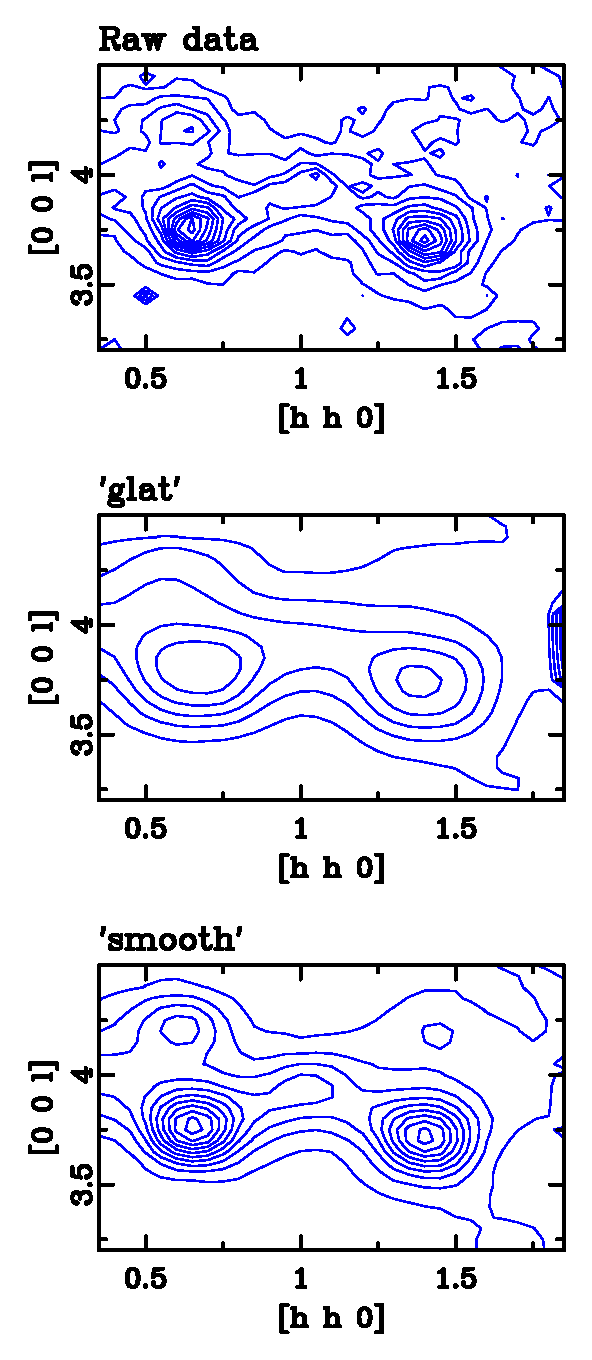
\includegraphics[scale=0.8]{mat.1.eps}
   \caption{Demonstration of data smoothing}
   \label{mat-fig1}
\end{figure}

{\it KUPLOT} has two different smoothing functions that can be used
for 1D as well as 2D data. The first type of smoothing is a simple
sliding average. The corresponding command is {\tt glat}. The name
is a reminder that the first {\it KUPLOT} version was in German
(smoothing in German is gl\"atten). The smoothing is performed by a
sliding average of $n$ neighboring points. The value of $n$ is given
as parameter of the command {\tt glat}. An example for the smoothing
operation is given in Figure \ref{mat-fig1}. The top view graph
shows the raw data showing quite noisy contour lines. The picture
below shows the same data after the data set was smoothed with a
value of $n=7$ using the command {\tt glat 1,7} assuming the values
are stored as data set one. It is apparent from Figure
\ref{mat-fig1} that this type of averaging broadens the peaks and
does not preserve the peak heights. An alternative way to smooth
data implemented in {\it KUPLOT} is the Savitzky-Golay algorithm
which is in principle a weighted sliding average. The weight is
given by a polynomial of user definable order (the default is 2).
The command for the later type of smoothing is {\tt smooth} with
parameters identical to {\tt glat}. However, the minimum number of
$n$ is five. The bottom view graph in Figure \ref{mat-fig1} was
smoothed with $n=7$ using the command {\tt smooth}. It can be
clearly seen that the widths and heights of the peaks are much
better preserved. For a detailed discussion about the smoothing
algorithm and its limits see e.g. Numerical Recipes by Press,
Flannery, Teukolsky \& Vetterling, Cambridge University Press, 1989.
\par

As a default, 2D data sets are per smoothed in x and y direction.
The user can restrict the smoothing to only one direction by adding
the optional parameter {\tt x} or {\tt y} to the {\tt glat} or {\tt
smooth} command. Again the reader might refer to the online help for
more detailed information on the smoothing commands.


\subsection{Sorting data \label{mat-sort}}

The command {\tt sort ik} will sort the data points in data set {\tt
ik} by increasing $x$ values. No other sorting is currently
implemented in {\it KUPLOT}, however one might implement any sorting
algorithm using the FORTRAN interpreter of the program.


\subsection{Rebinning data \label{mat-rebin}}

Sometimes a data set needs to be transformed onto a different grid
of $x$ or $x,y$ values. This is usually referred to as rebinning.
The most common application is to transform a data et from an
irregular grid to an equidistant grid. {\it KUPLOT} offers a
different mechanism for 1D and 2D data sets. The command {\tt rebin
ik, delta} will rebin the 1D data set {\it ik} to an equidistant
grid with a bin width of {\tt delta}. One needs to take care, that
the new grid is at least slightly larger than the original to
prevent 'holes' from appearing. In addition to an equidistant grid,
a data set can be interpolated on a set of $x$ values given by a
different data set. The command {\tt spline 1,2} for example would
interpolate data set one onto the $x$ values given by data set 2 and
store the result in a new data set.\par

To rebin a 2D data set, one needs to first save it in $x,y,z$ or
{\tt gn} format. This data file is then load back into {\it KUPLOT}
using the command {\tt load zz,file,dx,dy} and rebinned on the
desired grid {\tt dx, dy}. Obviously one can load $x,y,z$ files on
an irregular grid the same way. \par


\subsection{Matching and merging data sets \label{mat-merge}}

Sometimes two data sets differ by a scaling factor of an offset. The
command {\tt match} allows to find the scaling and/or offset that
gives the best agreement between two data sets. The scaling and
background is directly applied. Note that this function only works
for data sets, that have identical points in $x$. The command {\tt
merge} allows one to combine data sets. Points with common
$x$-values are averaged.

%------------------------------------------------------------------------

\section{Data manipulation using variables \label{mat-var}}

A very flexible way to manipulate data is the use of variables.
Details about the FORTRAN style interpreter and the usage of
variables were discussed in chapter \ref{fort}. Two simple examples
are given here for illustration. \par

In the first example we assume having a data set containing measured
intensities as function of some angle $\omega$. The following {\it
KUPLOT} commands will create values for $\sigma_{y}$ according to the
relation $\sigma_{y}(i) = \sqrt{y(i)}$.

\begin{MacVerbatim}
     1  do i[1]=1,np[1]
     2    dy[1,i[1]]=sqrt(y[1,i[1]])
     3  enddo
\end{MacVerbatim}

The first line starts a DO loop over all data points of data set
one, assuming that is where our data are stored. The variable {\tt
i[1]} is the loop control variable and {\tt np[1]} contains the
number of data points of data set one. For a complete list of
variables refer to section \ref{var} of this users guide. Next the
value of $\sigma_{y}$ for data point i[1] is computed (line 2). The
first parameter in {\tt dy[1,i[1]]} specifies data set one. Finally
(line 3) the loop is closed. The corresponding plot with the error
bars of the newly created values of $\sigma_{y}$ is shown in Figure
\ref{mat-fig2}.

\begin{figure}[!t]
   \centering
   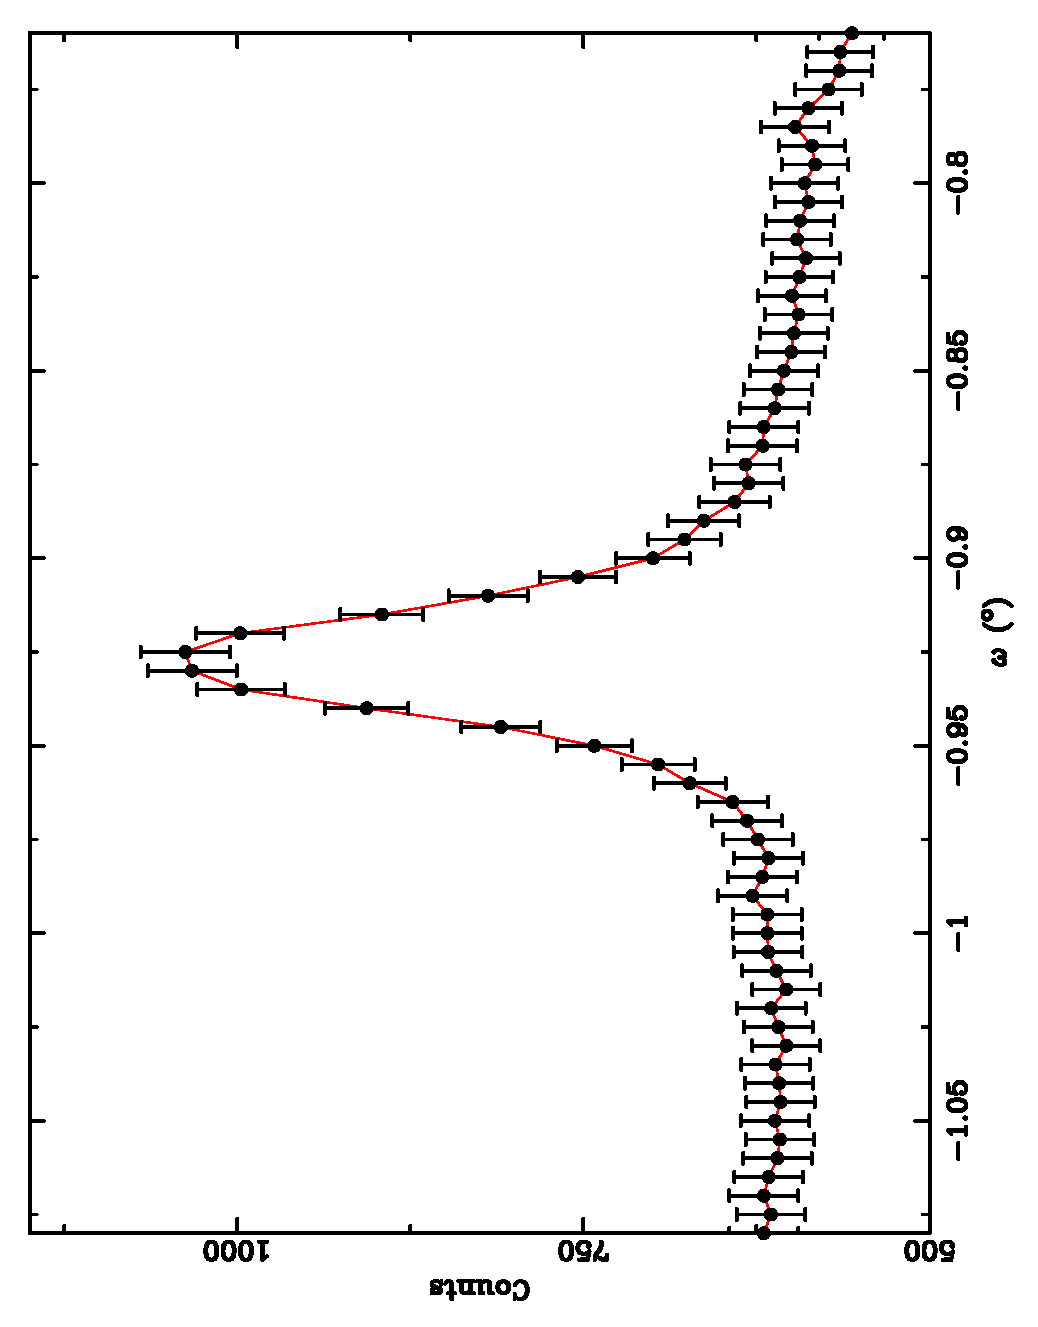
\includegraphics[scale=0.5, angle=270.0]{mat.2.eps}
   \caption{Plot of data manipulation example}
   \label{mat-fig2}
\end{figure}

The second example shows how to create a new data set using variables.
We assume that we have two data sets loaded, both having the same length
and identical x-values. We want to create a new data set with
the same x-values and y-values that are the average of the y-values of
the two load data sets, thus $y_{i}'''=\frac{1}{2}(y_{i}''+y_{i}')$.
Here $y'''$ stands for the new data set whereas $y''$ and $y'$
represent the values of the two loaded data sets. The {\it KUPLOT}
commands for our task are listed below:

\footnotesize
\begin{MacVerbatim}
     1  alloc aver.xy,np[1]
     2  #
     3  do i[1]=1,np[1]
     4    x[3,i[1]]=x[1,i[1]]
     5    y[3,i[1]]=0.5*(y[1,i[1]]+y[2,i[1]])
     6  enddo
\end{MacVerbatim}
\normalsize

First we have to allocate space for the new data set. This is
normally done by the command {\tt load} or {\tt func}, but the
command {\tt alloc} allows the user to create an empty data set,
just what we need here. The name {\it aver.xy} given as parameter to
the {\tt alloc} command in line 1 is the internal name for the data
set, e.g. showing up in the top left corner of the plot or when
using the {\tt show} command. This is an arbitrary name and {\bf no}
file of that name needs to exist. The second parameter specifies the
size of the new data set, in out case the same size as data sets one
(variable {\tt np[1]}) or two. Next we have a loop as in the
previous example over all data points (line 3). In lines 4--5 the
$x$- and $y$-values of the new data set number 3 are computed. Since
we assumed that both original data sets have the same $x$-values, we
just use one of them as $x$-values for the new set. Finally the loop
is closed (line 6).
\par

Although the usage of variables allows one to perform the same
functions as the {\tt ccal} and {\tt kcal} commands, the usage of
variables is much slower especially for large data sets and should
only be used if no corresponding build-in function is available.

%------------------------------------------------------------------------

\section{Data analysis \label{mat-anal}}

This section describes the data analysis functions of {\it KUPLOT}.
Apparently variables can also be used to calculate averages and
analyze data sets. The contents of a variable or result of an
expression can be displayed with the command {\tt eval}. Another
wide area of data analysis is to fit a theory function to a data
set. The least square fitting functions of {\it KUPLOT} are
discussed in the next chapter. As example for this chapter we use a
subsection of the diffuse scattering data displayed in previous
examples. The data are shown in Figure \ref{mat-fig3}. The circles
mark positions of maxima found in the data set by the command {\tt
smax}.

\begin{figure}[!t]
   \centering
   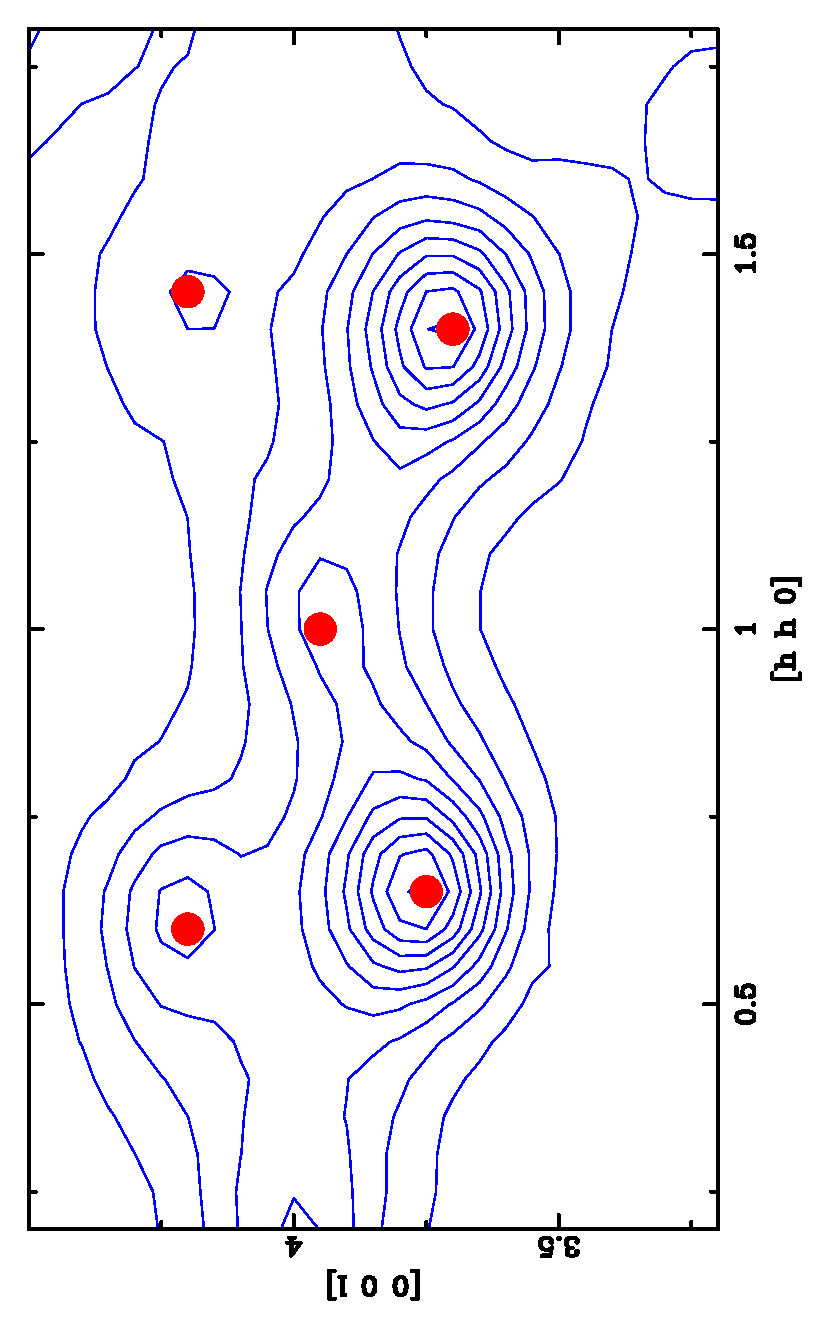
\includegraphics[scale=0.4, angle=270.0]{mat.3.eps}
   \caption{Marking of maxima within a plot}
   \label{mat-fig3}
\end{figure}

A maximum determined by {\tt smax} is defined as a point where all
$n$ neighboring points have smaller $y$- or $z$-values compared to
the reference point. The value of $n$ is the second parameter of the
{\tt smax} command, the first is the data set number. The maxima
marked in Figure \ref{mat-fig3} were determined with {\tt smax 1,3}
assuming we are dealing with data set one. The command {\tt ptyp}
allows one to select a symbol analog to {\tt mtyp} to mark the
positions of the determined maxima. Furthermore the positions of the
found maxima are displayed on the screen. The output for our example
is shown below:

\begin{MacVerbatim}
   Found maxima data set   1 (ifen =   3) :

      No.        pos. x       pos. y         value
      --------------------------------------------------
        1         .600        4.200             272.778
        2         .650        3.750             567.111
        3        1.000        3.950             273.889
        4        1.400        3.700             509.667
        5        1.450        4.200             156.778
\end{MacVerbatim}

You might verify these coordinates as the marked positions in figure
\ref{mat-fig3}. Other functions allow the user to determine the
integral or mean values of a given area of the data set.\par

Next we will determine the integral of the left diffuse peak in
figure \ref{mat-fig3}. This is done using the command

\begin{MacVerbatim}
    inte 1, .423750, .903750, 3.4716, 3.99168
\end{MacVerbatim}

The first parameter specifies the data set number followed by the area
to be integrated given as $x_{min}, x_{max}, y_{min}$ and $y_{max}$.
If those last 4 parameters are omitted, the complete current plotting
window is used. The screen output of this command is:

\footnotesize
\begin{MacVerbatim}
    Integration result for data set   1 :
       x-range    :    .4238     to    .9038
       y-range    :    3.472     to    3.992
       Integral   :    57.06     +-    .3650      (    100 pkt)
\end{MacVerbatim}
\normalsize

The command {\tt mean} with similar parameters can be used to
calculate mean values and standard deviations in the given region.
The region above was determined using the {\tt mouse} functions (see
\ref{mouse}).

%------------------------------------------------------------------------

\section{Fourier transform \label{mat-four}}

{\it KUPLOT} can calculate a discrete Fourier transform of a 1D or
2D data set. Let us start with a little mathematics first. Details
can again be found in the Numerical Recipes. The function we want
to Fourier transform is $f(x_{i})$ with $i=1,..N$ with a constant
grid size of $\Delta x$. This gives us the following range in Fourier
space:

\begin{equation}
  h_{n} = \frac{n}{N \Delta x} \;\; \mbox{with} \;\;
      n = -\frac{N}{2} .. \frac{N}{2}
  \label{mat-eq1}
\end{equation}

\noindent
The Fourier transform is calculate as

\begin{equation}
  F(h_{n}) = \Delta x \sum_{i=1}^{N} f(x_{i}) \left [
             \cos (2\pi h_{n}x_{i}) + i \sin (2\pi h_{n}x_{i}) \right ].
  \label{mat-eq2}
\end{equation}

\begin{figure}[!t]
   \centering
   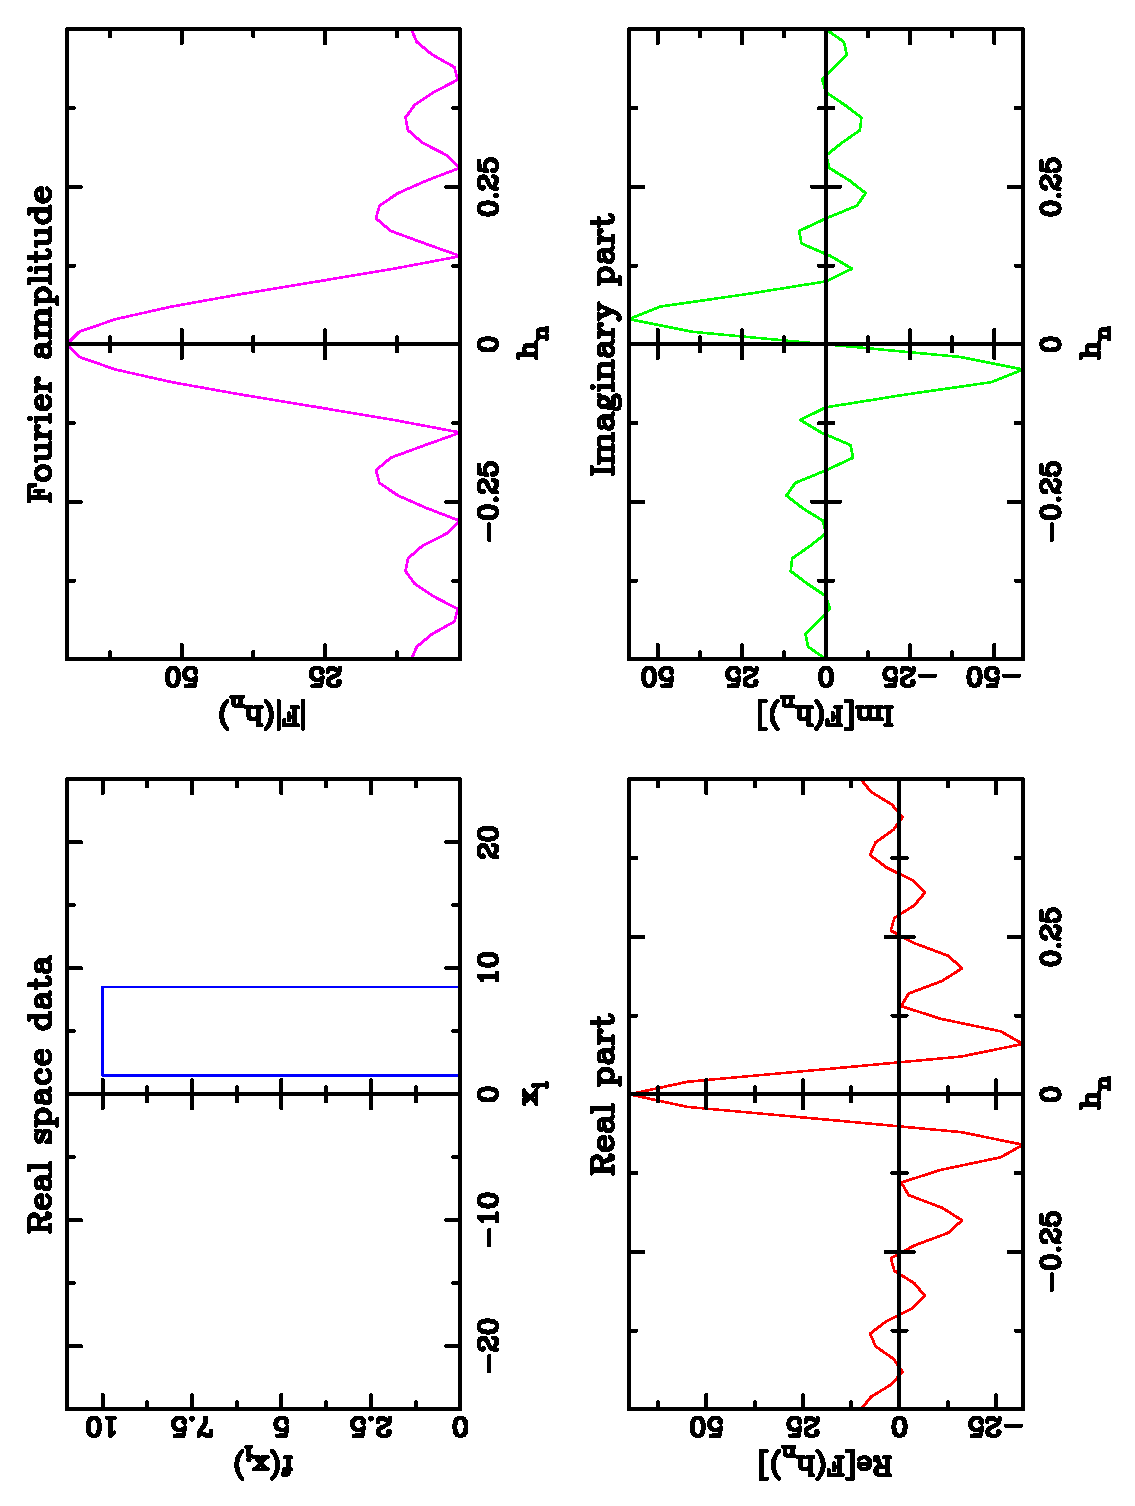
\includegraphics[scale=0.5, angle=270.0]{mat.4.eps}
   \caption{Fourier transform of box function}
   \label{mat-fig4}
\end{figure}

The Fourier transform is a complex quantity and {\it KUPLOT} allows one
to select the real and imaginary part and/or amplitude and phase angle
to be stored as new data sets. \par

Let us consider a simple example, a box function as displayed in the
upper left panel of Figure \ref{mat-fig4}. Our data set has $N=50$
points and a grid size of $\Delta x = 1.0$. Using equation \ref{mat-eq1}
we find the grid size in Fourier space to be $1/50 = 0.02$ and a
calculated range of $-1/2\Delta x = -0.5$ to $0.5$. In our example
the command for the calculation of the Fourier transform is:

\begin{MacVerbatim}
  four ria
\end{MacVerbatim}

The parameter {\tt ria} specifies that we want to keep the {\bf
r}eal and {\bf i}maginary part as well as the {\bf a}mplitude of the
Fourier transform. All three parts and the box function are shown in
Figure \ref{mat-fig4}.


%------------------------------------------------------------------------

\section{Other functions \label{mat-other}}

The command {\tt deriv ik,n} will calculate the numerical n-th
derivative of data set {\tt ik} and store the result a a new data
set. The convolution of two data sets can be calculated using the
command {\tt conv}. Both data sets need to have a common equidistant
set of $x$ values. 
